\chapter{Benchmark \& Discussion}

In this chapter the three algorithms are benchmarked with different parameters and scenarios. The first series of tests is conducted in a static environment for a basic understanding of the algorithm performance and the second series is held in various dynamic settings to explore the dynamic capabilities of the algorithms. The testing environment was the minion cluster of the departement of Informatics at the University of Zurich. The cluster consists of 16 machines and each machine has 128 GB RAM and two E5-2680 v2 at 2.80GHz processors. Every processor has 10 cores and the interlink between the machines is a 40Gbps Infiniband setup. The cluster has different partition speeds (slow, fast, superfast). All tests were conducted on superfast partitions.

\section{Results I: Algorithms Performance in Static Environments}

\subsection{Solution Quality over Time}

The main focus of the work has been on the performance of the algorithms in terms of solution quality over time.  In this section, the three algorithms are going to be compared on their behaviour and the influence of the parameters density, number of agents and run mode (synchronous/asynchronous) in terms of this attribute.

\begin{figure}[H]
\centering
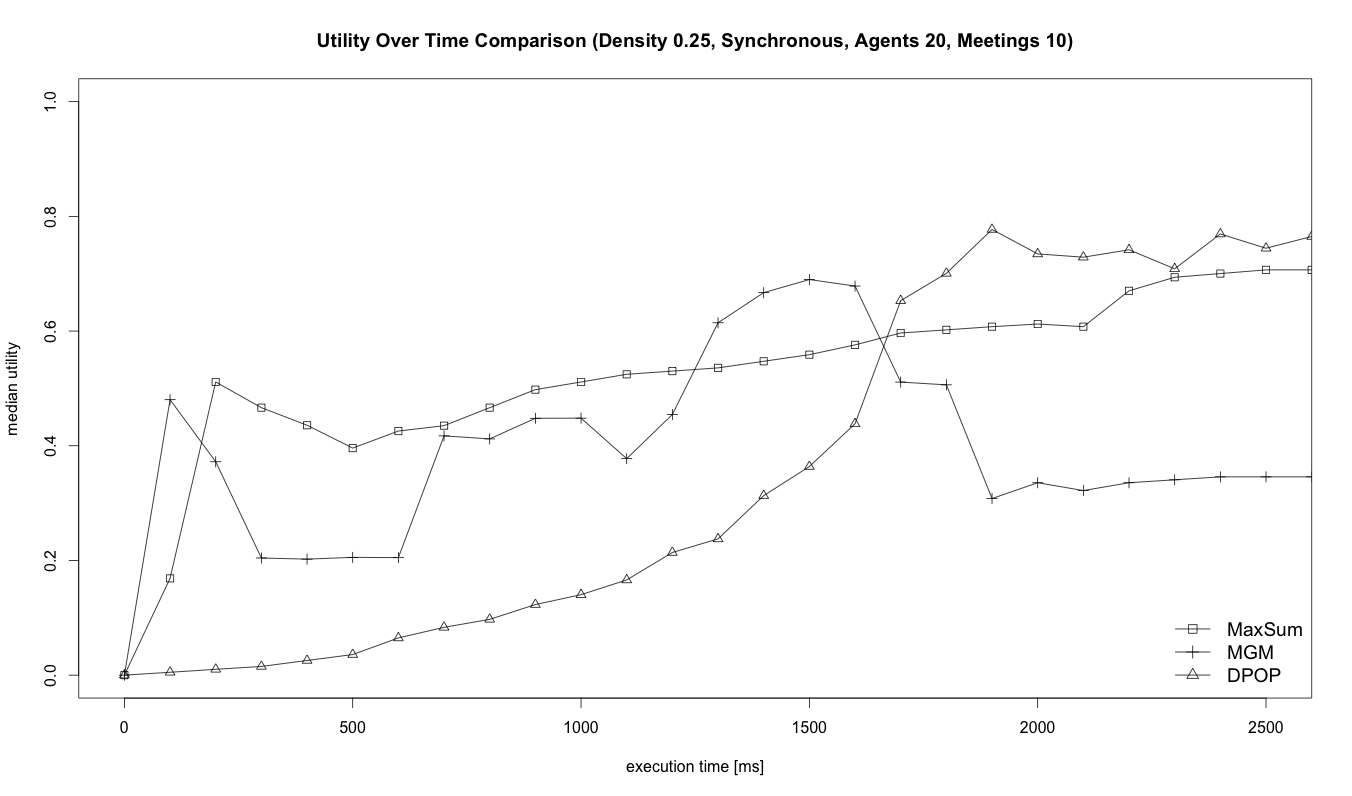
\includegraphics[width=350px]{graphics/experiments/static/st_1}
\caption{Utility over Time Comparison (Density 0.25, Synchronous, Agents 20, Meetings 10)}
\label{fig:st1}
\end{figure}

\begin{figure}[H]
\centering
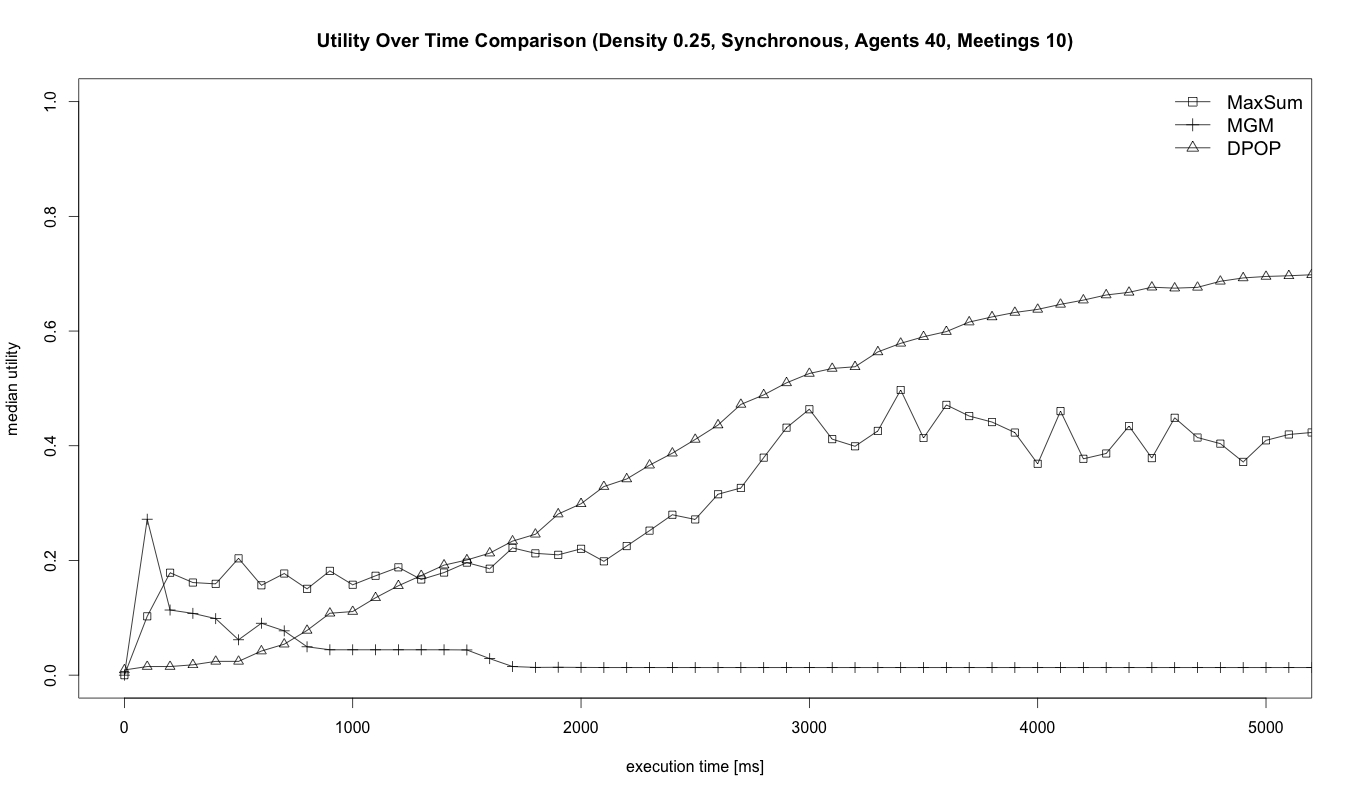
\includegraphics[width=350px]{graphics/experiments/static/st_3}
\caption{Utility over Time Comparison (Density 0.25, Synchronous, Agents 40, Meetings 10)}
\label{fig:st2}

\end{figure}

% ----------------------------
One can see in the figure \ref{fig:st1} and \ref{fig:st2} that the algorithms do show the expected performance at the start of the benchmark. MGM and MaxSum both increase quite fast at the beginning of the run, whereas MGM increases a bit faster. Because the algorithms do not always converge, the mean utility in the end is lower compared to DPOP. The MaxSum Algorithm shows the stronger performance in regards of convergence and quality of solution than MGM. In figure \ref{fig:st2} one can see the sometimes erratic behaviour of the MGM algorithm. This could well be a problem with the implementation instead of the algorithm itself. The DPOP algorithm shows a steady increase with a slow start as it was expected. By increasing the number of agents, the time to reach a certain level of quality increases for all three algorithms. A further measurement for quality has been created as a combination of the percentage of accordance on a meeting time and the percentage of overlaps in an agents schedule. The figures can be found in the appendix (Figure \ref{fig:st_2}, Figure \ref{fig:st_3}) as they are quite similar to the utility benchmarks.

TABLE HERE

% --------------------------

\begin{figure}[H]
\centering
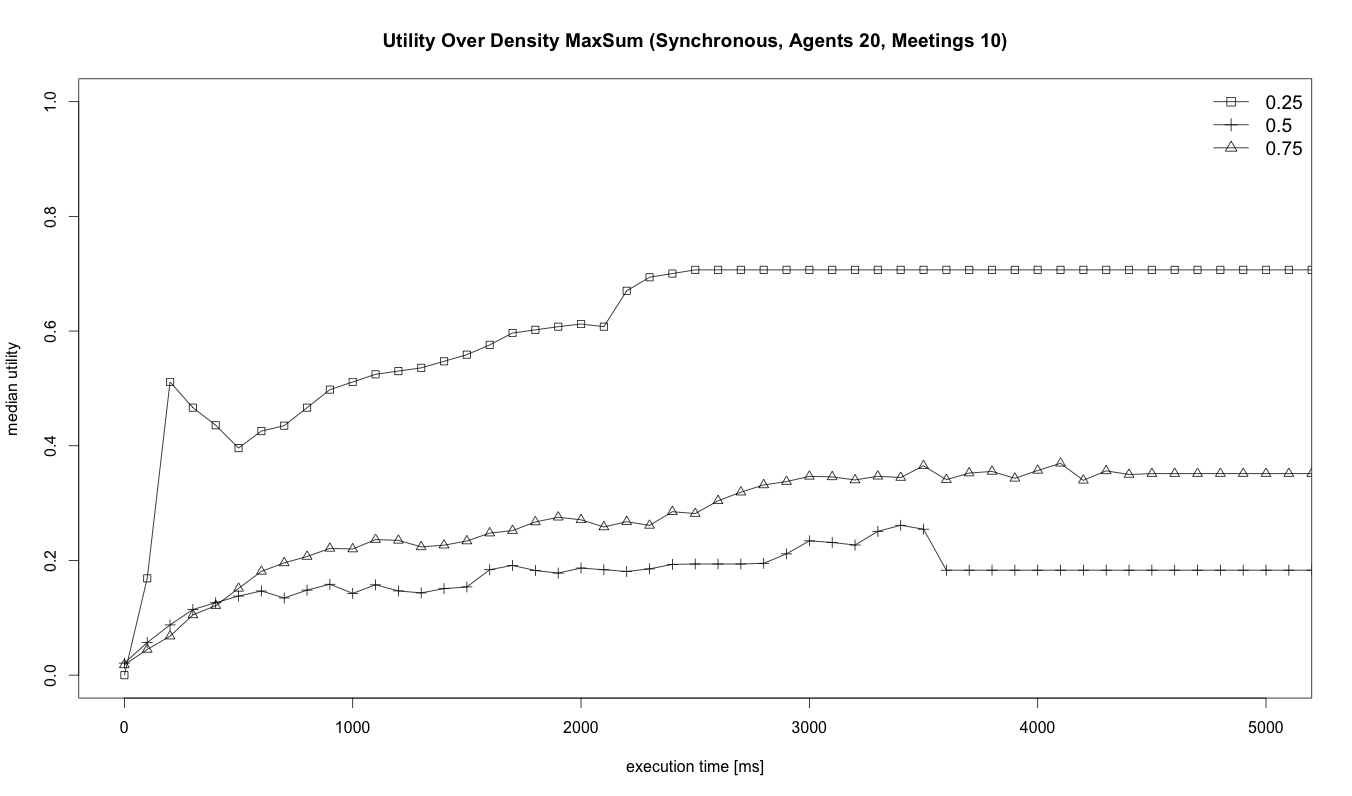
\includegraphics[width=330px]{graphics/experiments/static/st_5}
\caption{Utility over Density MaxSum (Synchronous, Agents 20, Meetings 10)}
\label{fig:st_5}
\end{figure}
\begin{figure}[H]
\centering
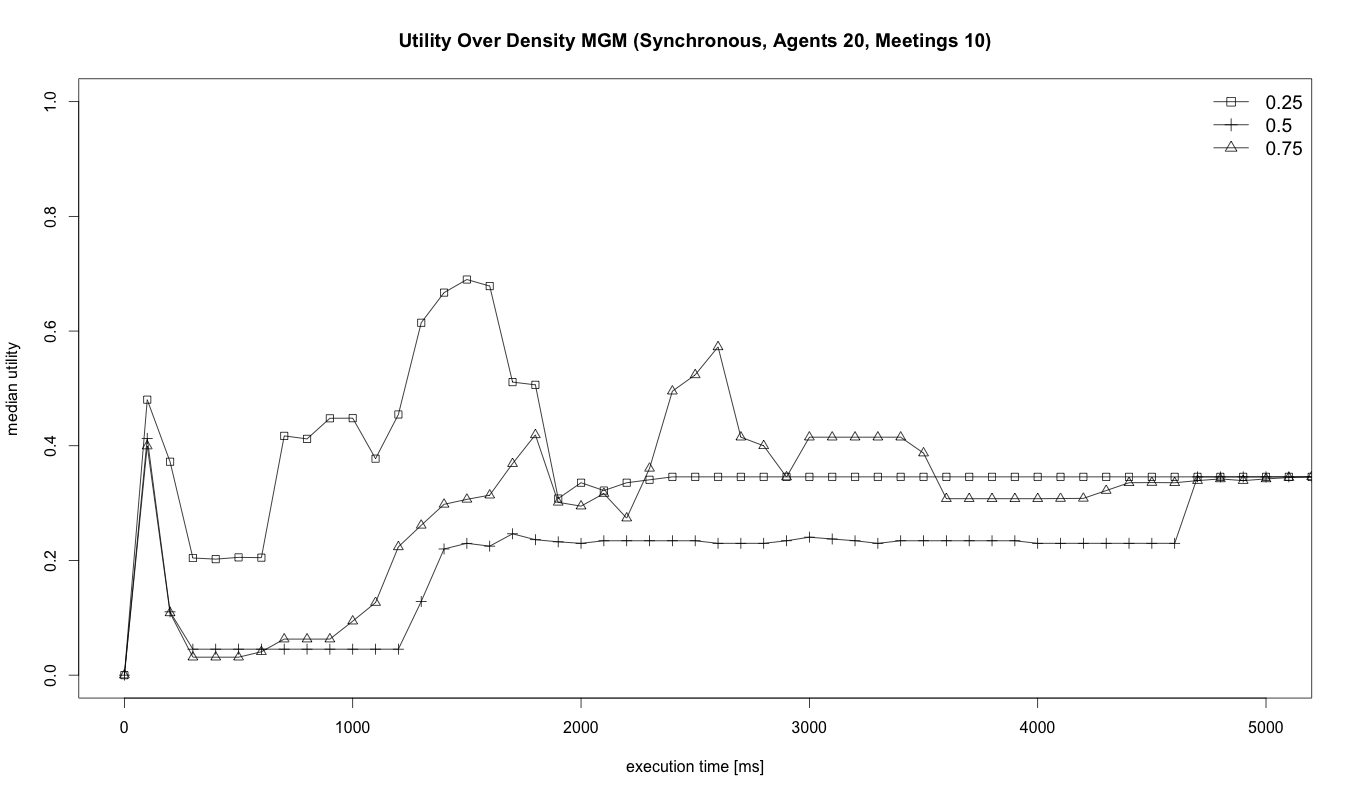
\includegraphics[width=330px]{graphics/experiments/static/st_6}
\caption{Utility over Density MGM (Synchronous, Agents 20, Meetings 10)}
\label{fig:st_6}
\end{figure}
\begin{figure}[H]
\centering
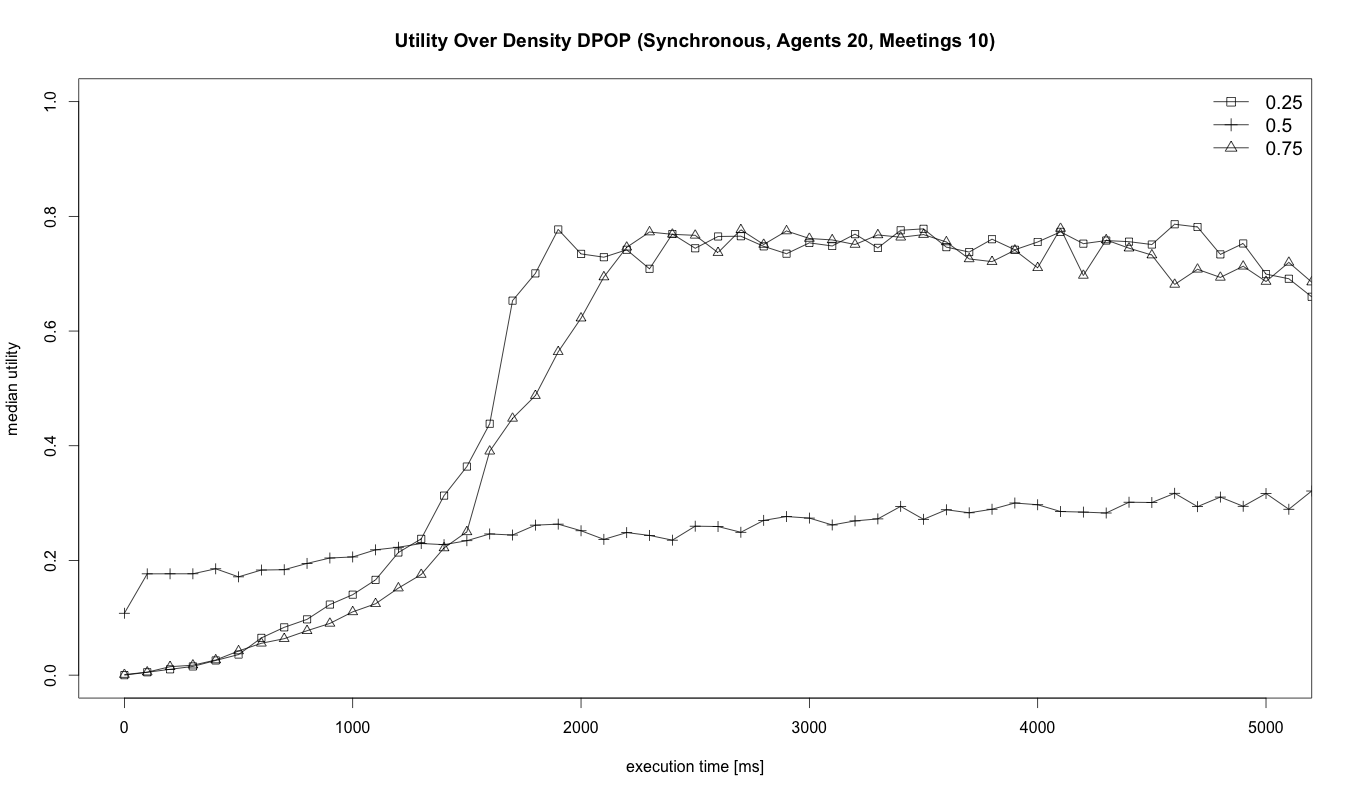
\includegraphics[width=330px]{graphics/experiments/static/st_7}
\caption{Utility over Density DPOP (Synchronous, Agents 20, Meetings 10)}
\label{fig:st_7}
\end{figure}

% ----------------------------
Density has been defined as the number of blocked timeslots in the participations schedules. One would expect this density parameter to have a linear effect and decrease the median utility as higher as the value is set. The figures \ref{fig:st_5}, \ref{fig:st_6}, \ref{fig:st_7}  present a rather different image. The value with the most impact has been 0.5, 0.25 and 0.5 have performed quite similar. This is especially the case with the DPOP algorithm. It is suspected that this is a specific property of the meeting scheduling problem as the density parameter on one hand opens up many timeslots by having a low number of blocked timeslots and on the other hand favors a few not blocked slots on high percentages.

%-----------------------------
\begin{figure}[H]
\centering
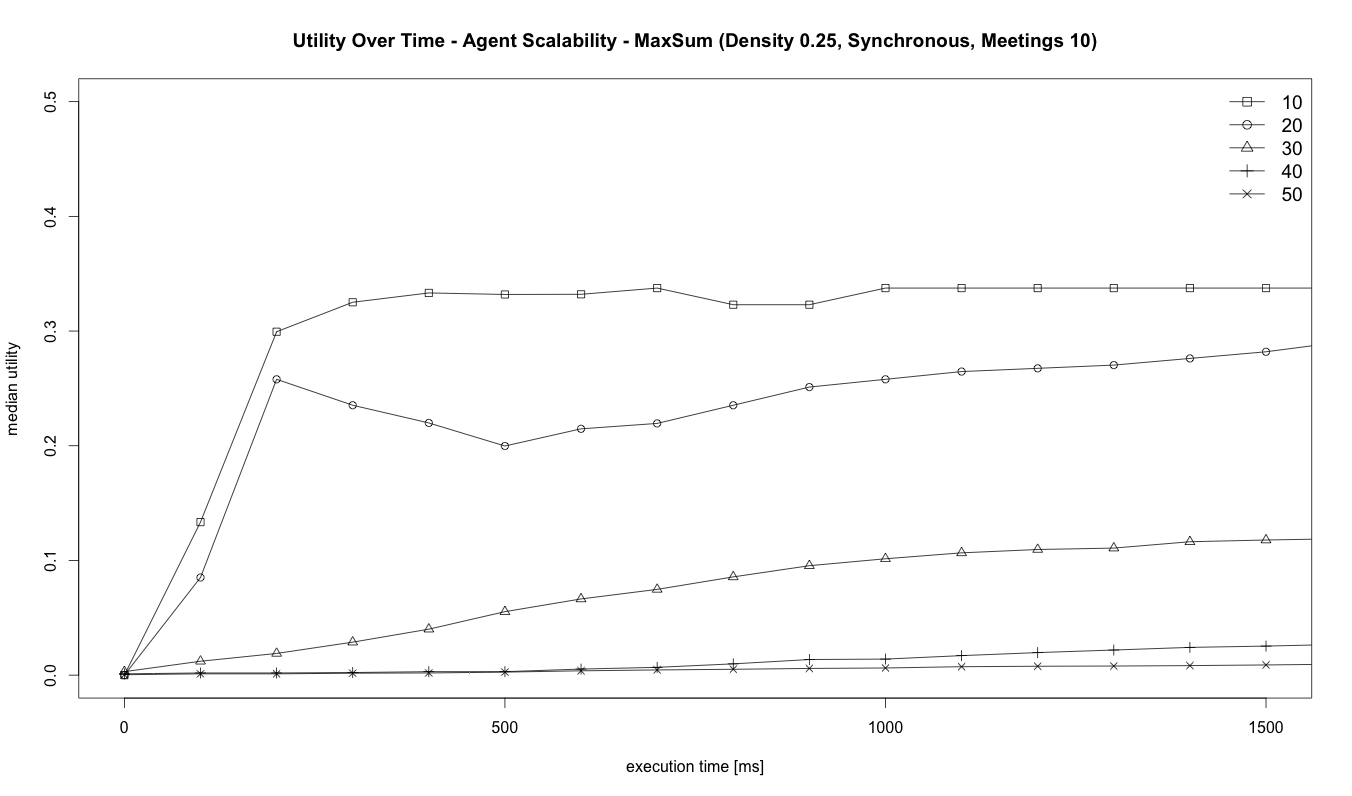
\includegraphics[width=330px]{graphics/experiments/static/st_8}
\caption{Utility over Time - Agent Scalability - MaxSum (Density 0.25, Synchronous, Meetings 10)}
\label{fig:st_8}
\end{figure}
\begin{figure}[H]
\centering
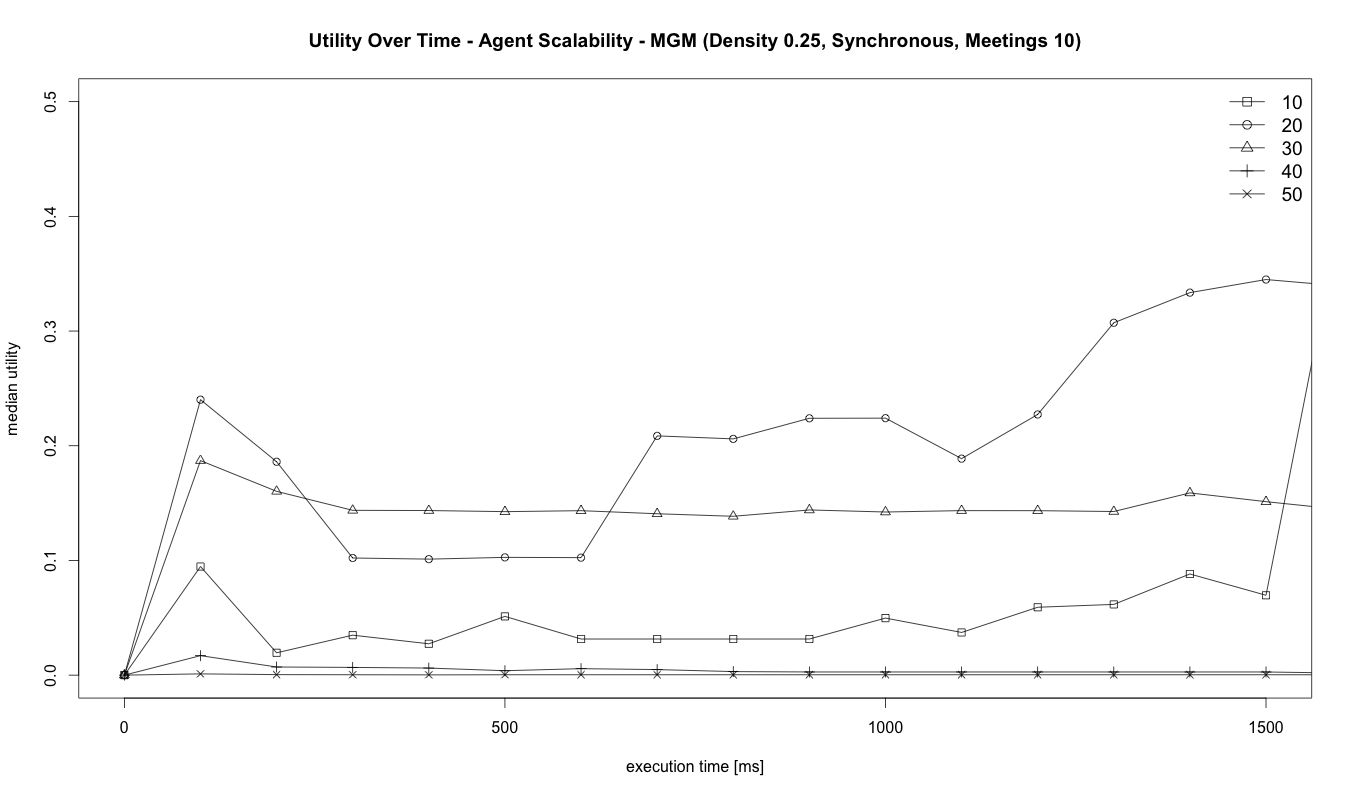
\includegraphics[width=330px]{graphics/experiments/static/st_9}
\caption{Utility over Time - Agent Scalability - MGM (Density 0.25, Synchronous, Meetings 10)}
\label{fig:st_9}
\end{figure}
\begin{figure}[H]
\centering
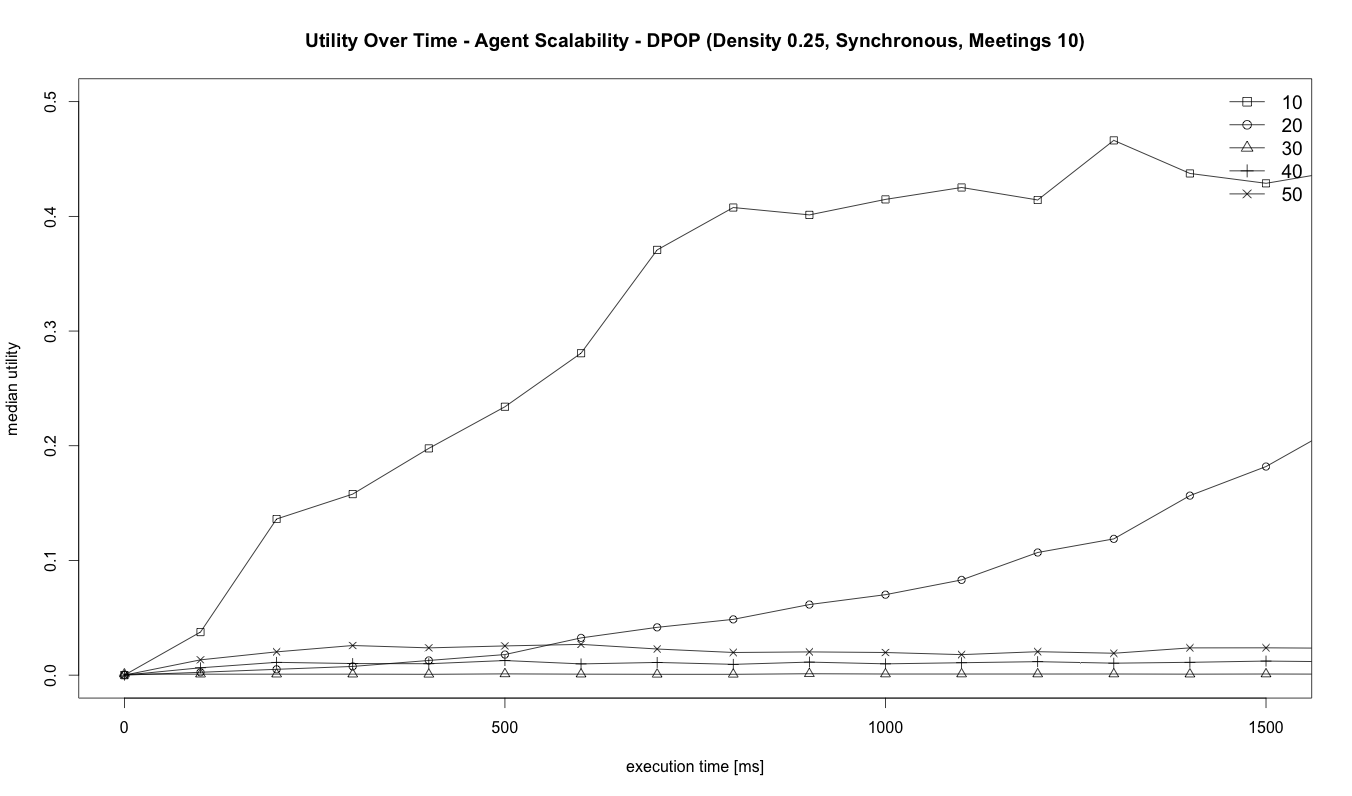
\includegraphics[width=330px]{graphics/experiments/static/st_10}
\caption{Utility over Time - Agent Scalability - DPOP (Density 0.25, Synchronous, Meetings 10)}
\label{fig:st_10}
\end{figure}

% ----------------------------
By testing the scalability of the algorithms on the number of agents with a fixed density and a fixed amount of meetings, it could be discovered that MaxSum scales fairly well and steadily (Figure \ref{fig:st_8}). MGM on the other hand again shows inconsistent behaviour, whereas the best performance can been seen with 20 agents (Figure \ref{fig:st_9}). For DPOP one can see that the time  to reach a certain quality increases drastically with added agents. This property has been expected due to the complexity increase in the messages with an increase of the graph size (Figure \ref{fig:st_10}).
%-----------------------------
\begin{figure}[H]
\centering
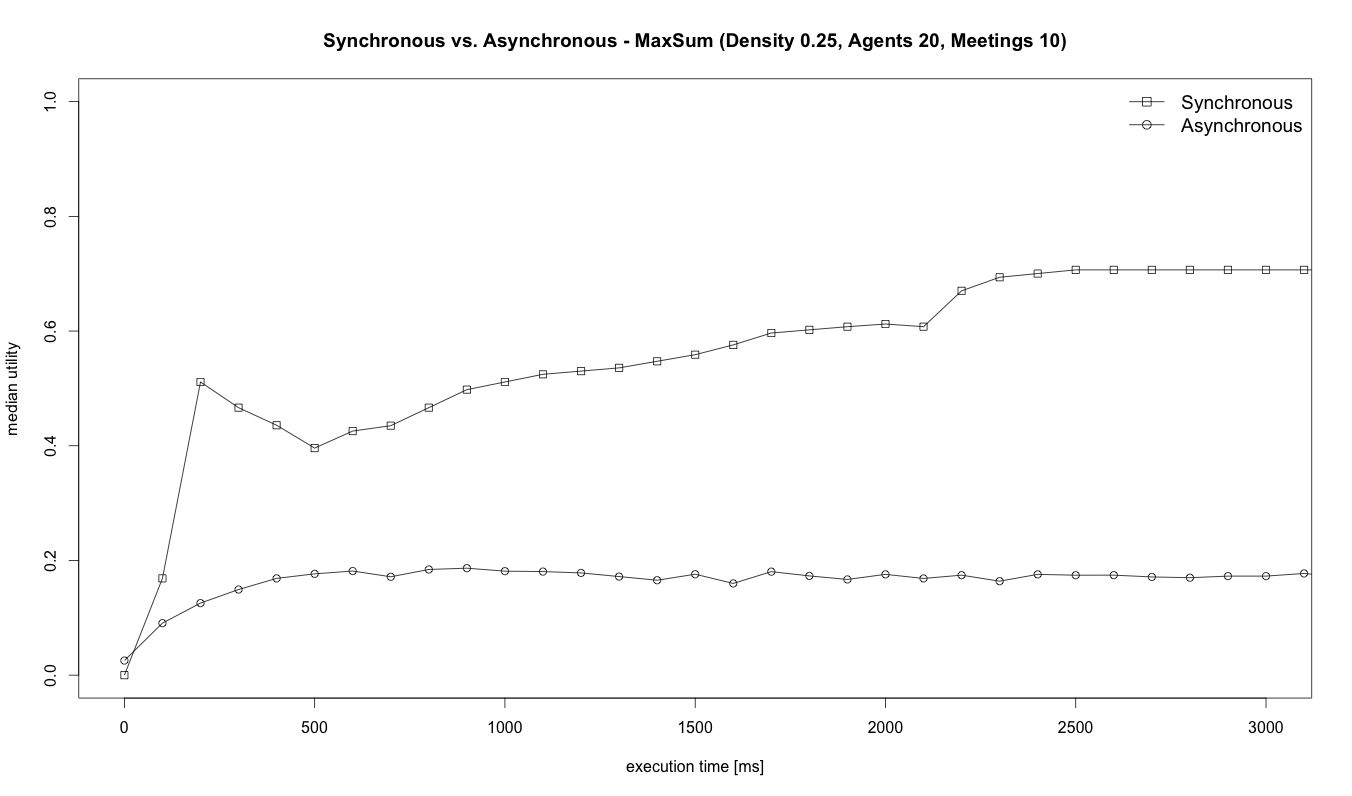
\includegraphics[width=330px]{graphics/experiments/static/st_11}
\caption{Synchronous vs. Asynchronous - MaxSum (Density 0.25, Agents 20, Meetings 10)}
\label{fig:st_11}
\end{figure}
\begin{figure}[H]
\centering
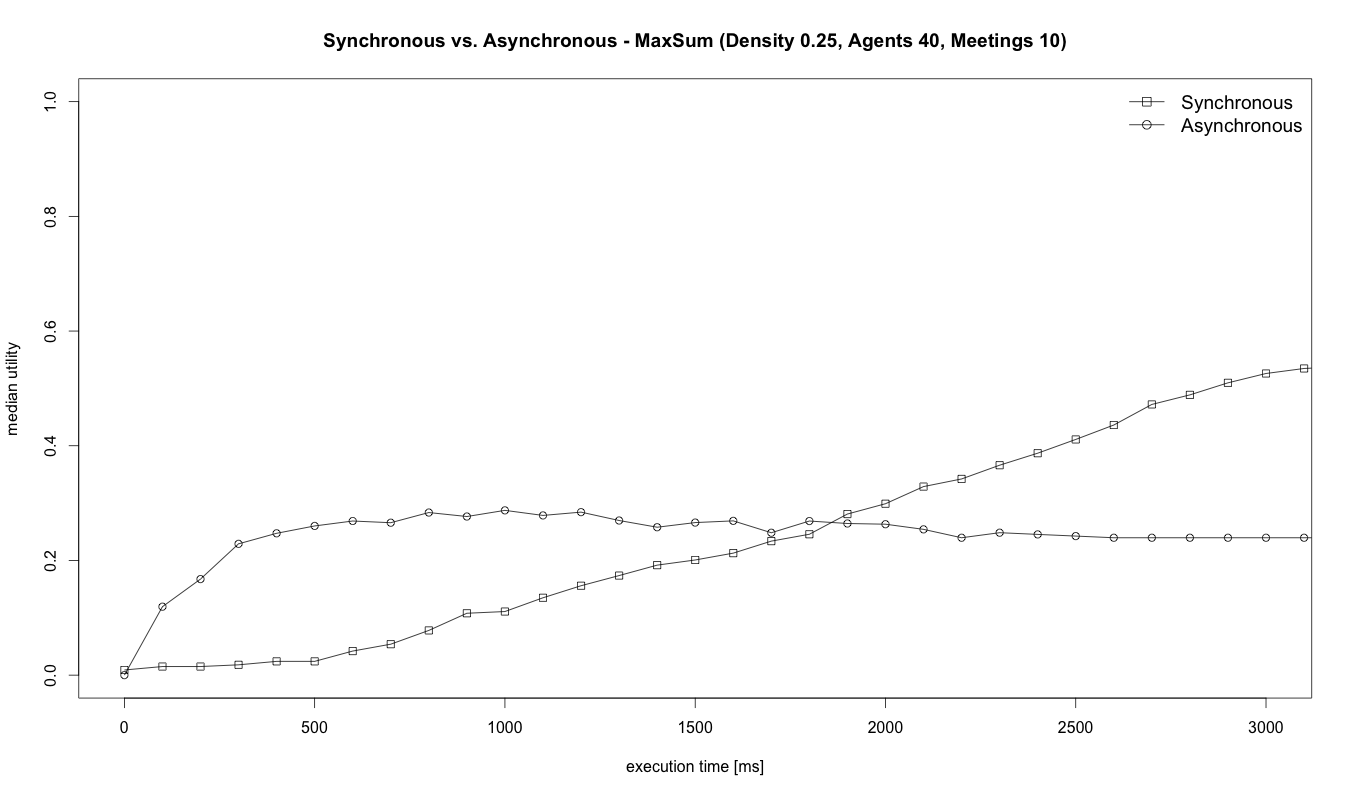
\includegraphics[width=330px]{graphics/experiments/static/st_12}
\caption{Synchronous vs. Asynchronous - MaxSum (Density 0.25, Agents 40, Meetings 10)}
\label{fig:st_12}
\end{figure}

% ----------------------------
An interesting property of MaxSum has been discovered by comparing the synchronous and asynchronous run mode. It seems that with low numbers of agents the performance of the synchronous mode is better at the start of a run, but the asynchronous variation is faster with increased amounts of agents (Figures \ref{fig:st_11}, \ref{fig:st_12}). The MaxSum algorithm shows some interesting scalability properties in asynchronous mode, which can also be seen in Figure \ref{fig:st_14}. MGM seems to converge faster in asynchronous mode on a low number of agents (Figure \ref{fig:st_12b}). DPOP does not seem to profit from the asynchronous mode and rather slows down (Figure \ref{fig:st_13}).
%-----------------------------

\begin{figure}[H]
\centering
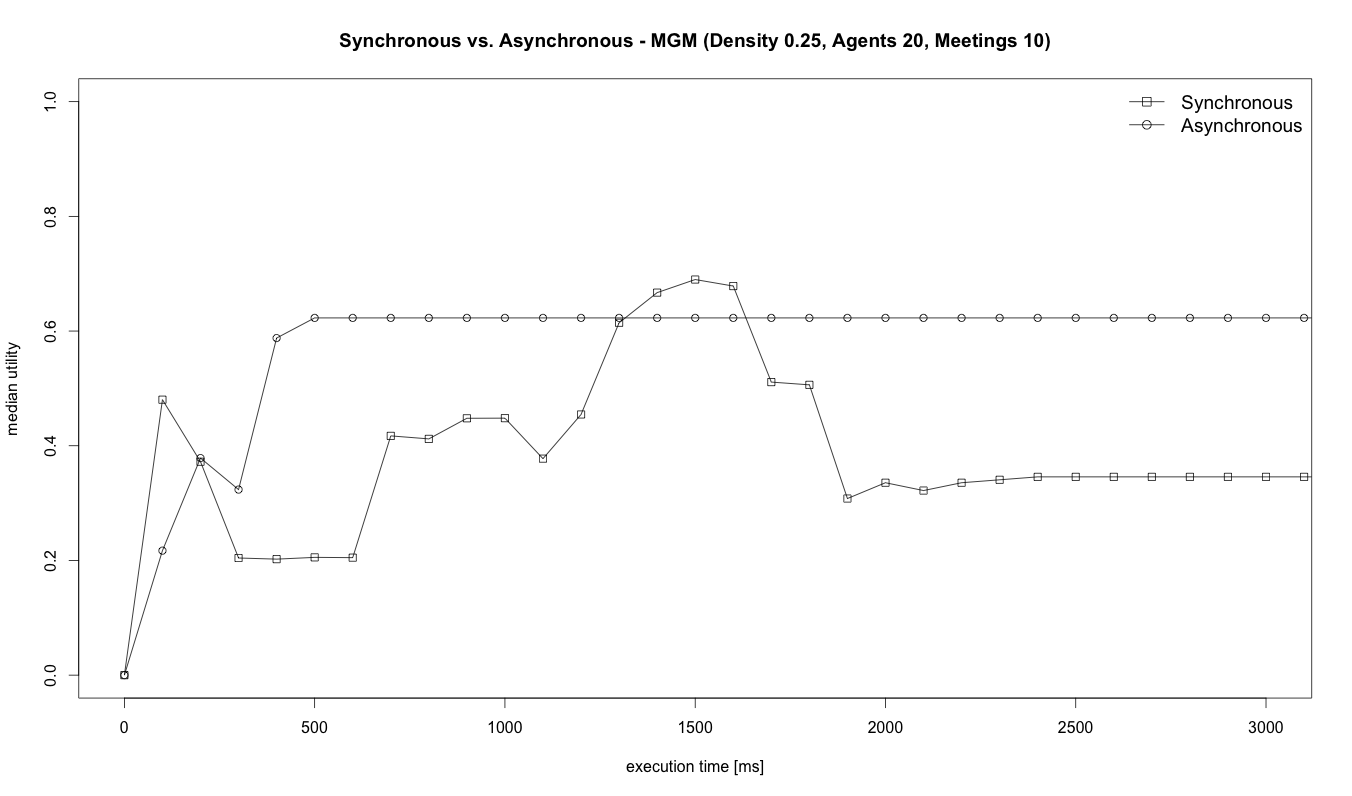
\includegraphics[width=330px]{graphics/experiments/static/st_12b}
\caption{Synchronous vs. Asynchronous - MGM (Density 0.25, Agents 20, Meetings 10)}
\label{fig:st_12b}
\end{figure}
\begin{figure}[H]
\centering
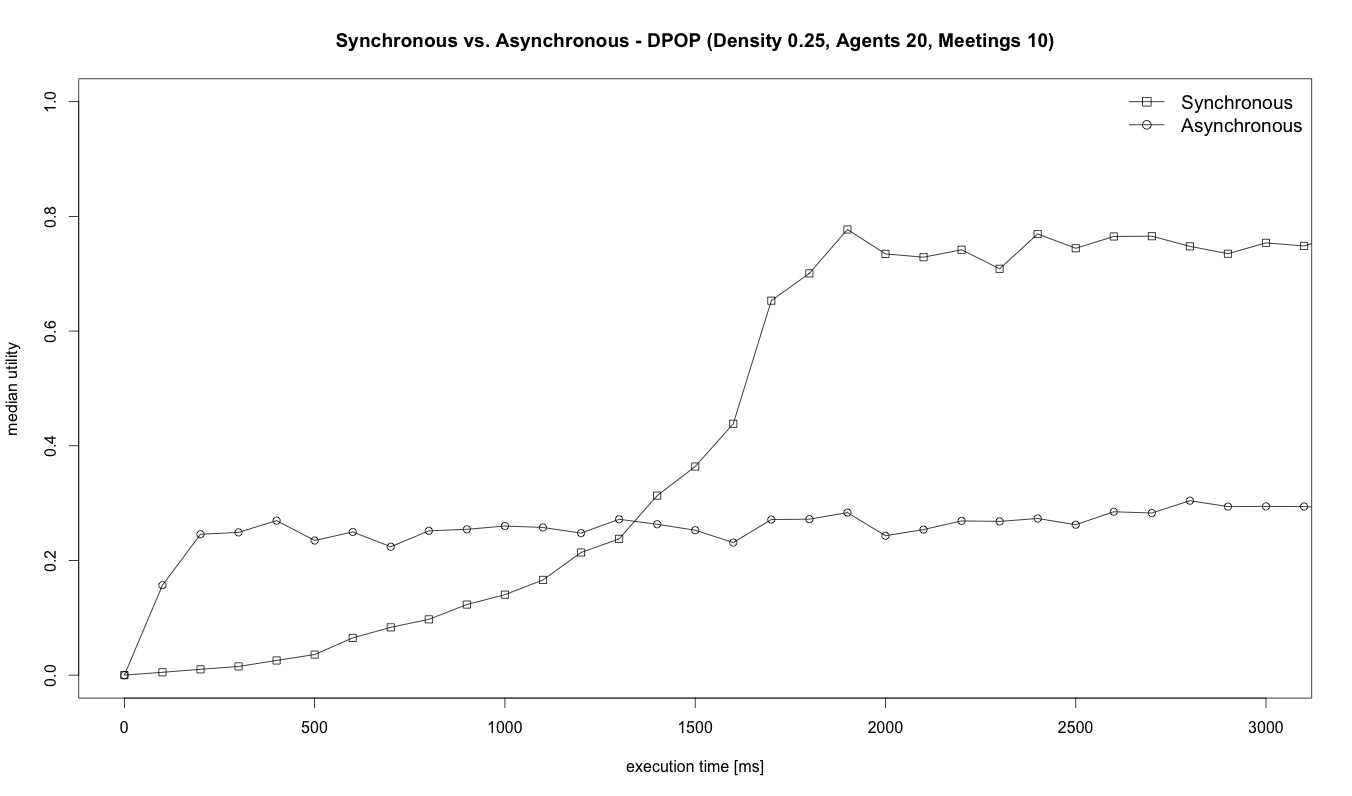
\includegraphics[width=330px]{graphics/experiments/static/st_13}
\caption{Synchronous vs. Asynchronous - DPOP (Density 0.25, Agents 20, Meetings 10)}
\label{fig:st_13}
\end{figure}


\subsection{Time to Convergence}

In this section, the time to convergence is going to be analyzed. The focus lays on the scalability properties of the algorithms in different densities and run modes (synchronous/asynchronous) in regards to agents. Meetings have, because of the participation limitation a limited influence on the performance of the algorithms when meeting numbers are increased. 

\begin{figure}[H]
\centering
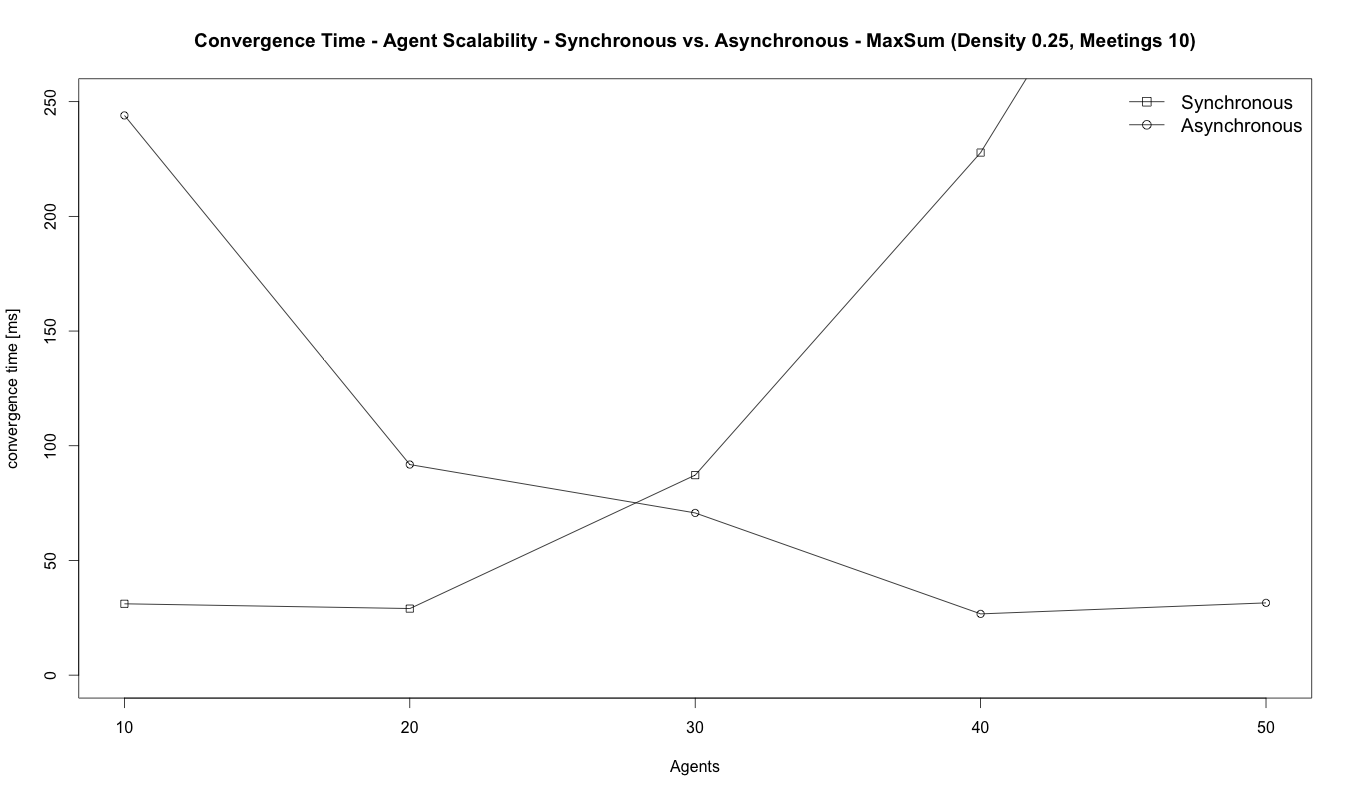
\includegraphics[width=230px]{graphics/experiments/static/st_14}
\caption{Convergence Time - Agent Scalability - MaxSum (Density 0.25, Meetings 10)}
\label{fig:st_14}
\end{figure}

\begin{figure}[H]
\centering
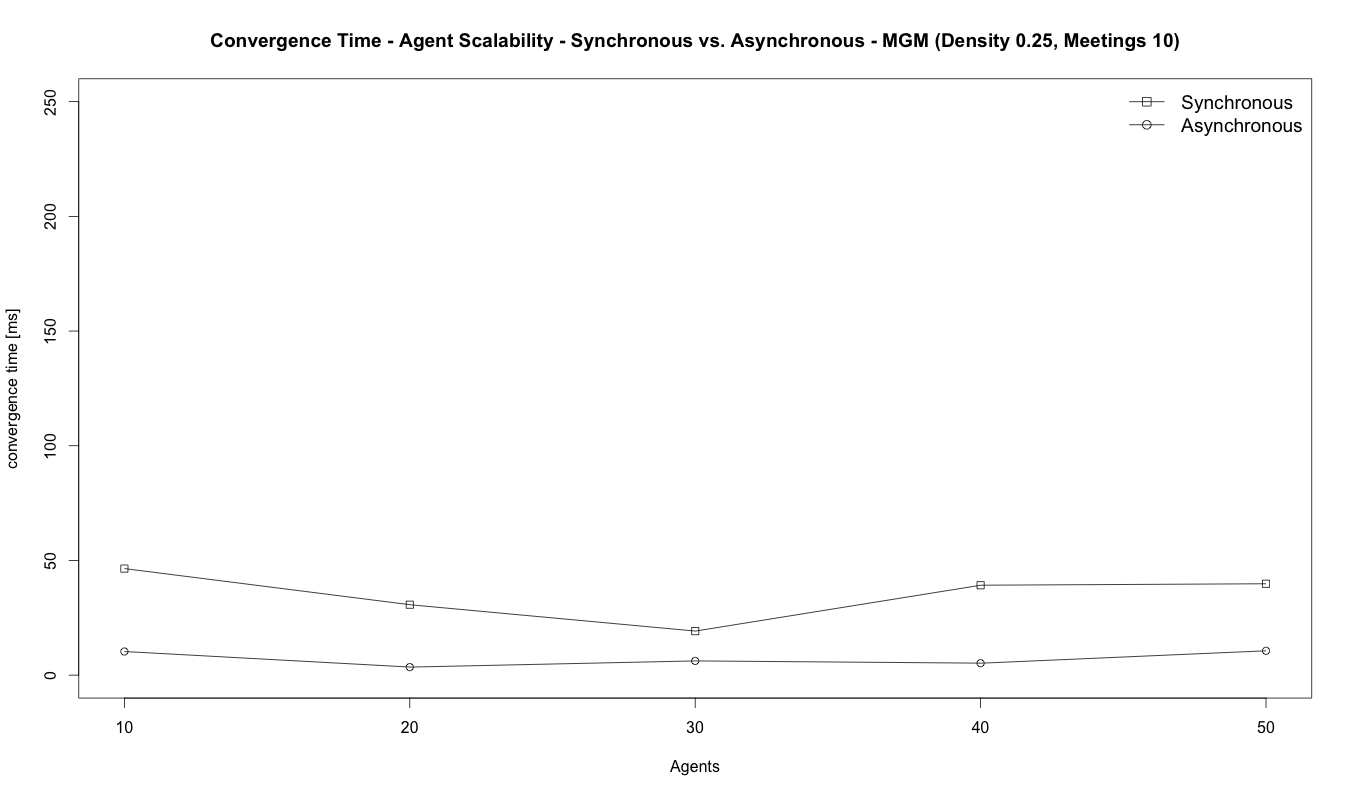
\includegraphics[width=230px]{graphics/experiments/static/st_15}
\caption{Convergence Time - Agent Scalability - MGM (Density 0.25, Meetings 10)}
\label{fig:st_15}
\end{figure}

\begin{figure}[H]
\centering
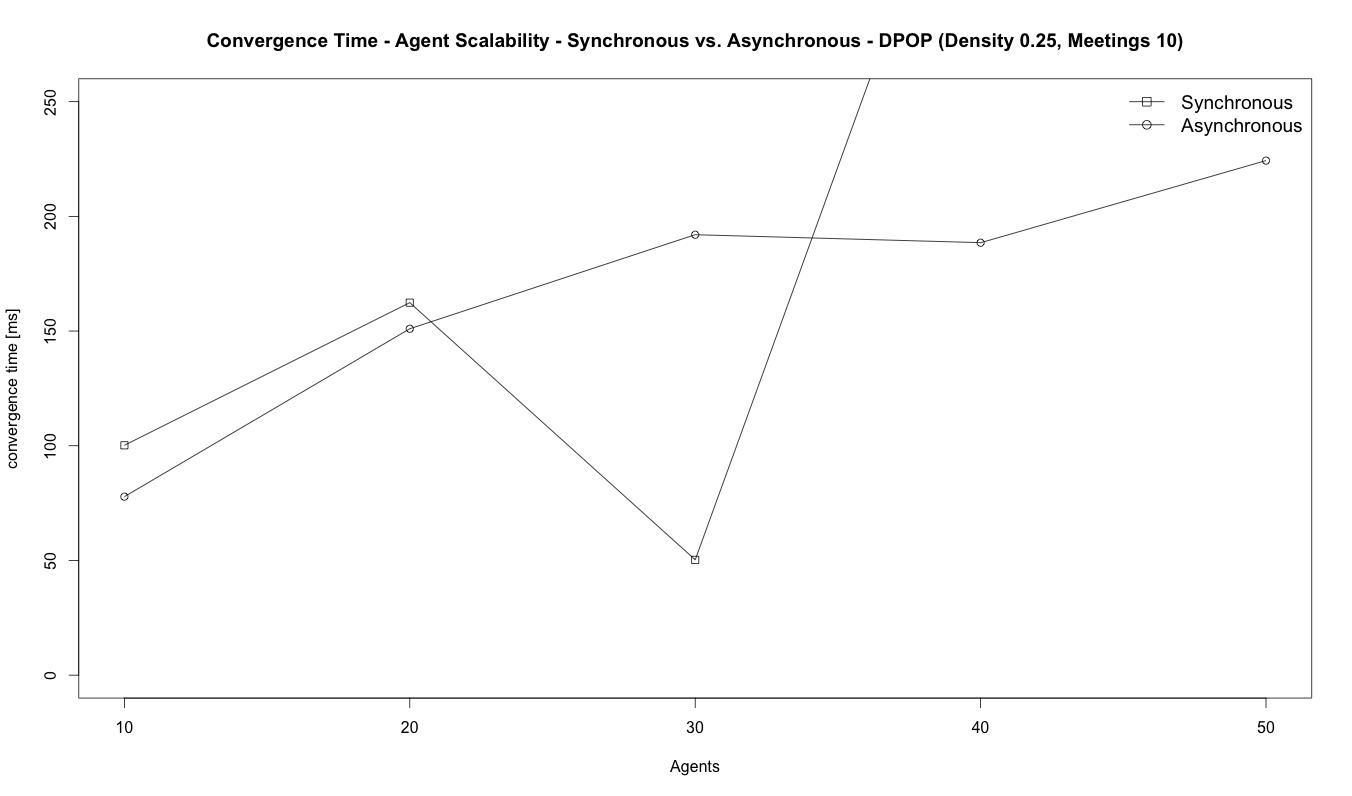
\includegraphics[width=230px]{graphics/experiments/static/st_16}
\caption{Convergence Time - Agent Scalability - DPOP (Density 0.25, Meetings 10)}
\label{fig:st_16}
\end{figure}

% ----------------------------
MaxSum again presents an obscure behaviour by actually converging faster in asynchronous mode with an increased number of agents. When run in synchronous mode, the algorithm shows slower convergence times with added agents (Figure \ref{fig:st_14}). The MGM algorithm does seem to profit from the asynchronous mode on increased amounts of vertices in the graph, as it stays very stable on a lower level of converges time than the synchronous variant (Figure \ref{fig:st_15}). DPOP, also seems to converge faster in asynchronous mode (Figure \ref{fig:st_16}).

TABLE HERE

%-----------------------------

\begin{figure}[H]
\centering
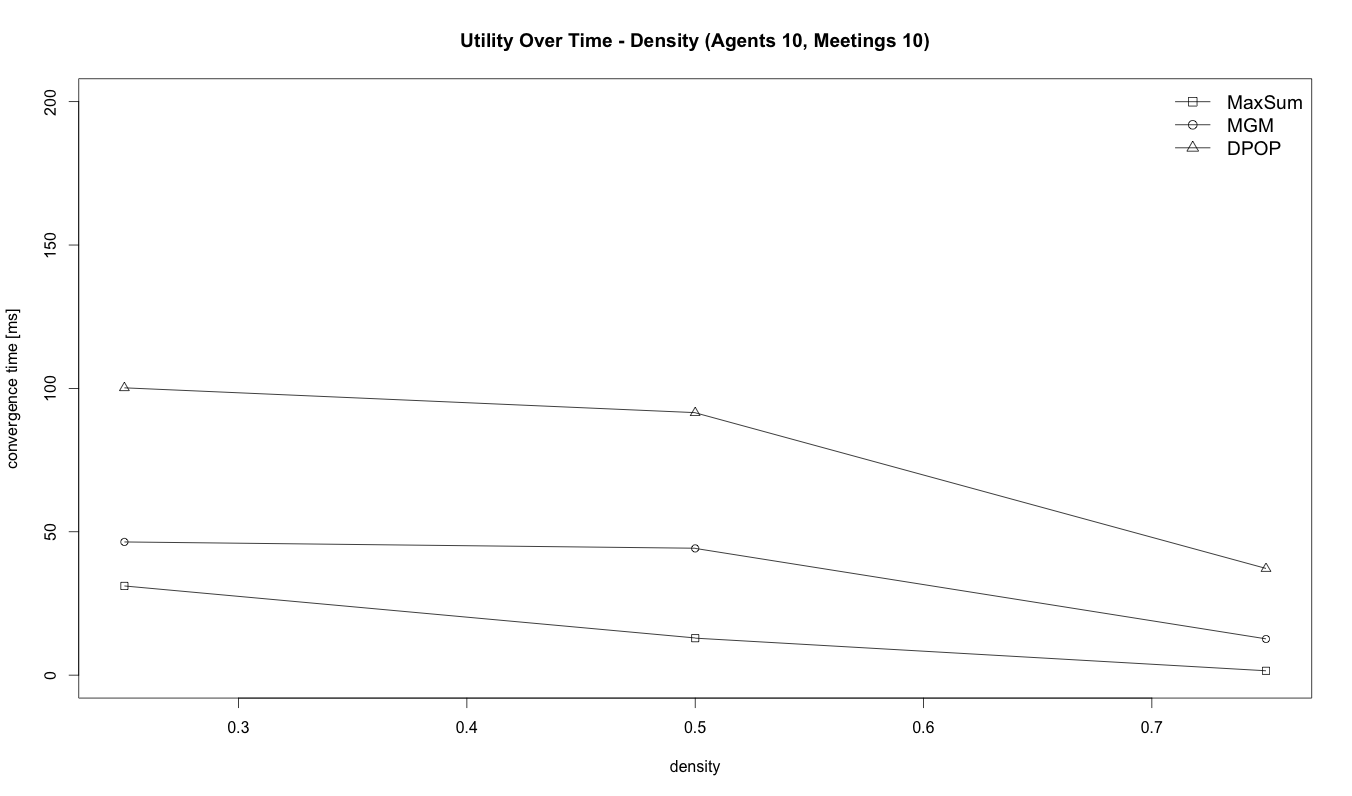
\includegraphics[width=330px]{graphics/experiments/static/st_17}
\caption{Utility over Time - Agents 10, Meetings 10}
\label{fig:st_17}
\end{figure}

\begin{figure}[H]
\centering
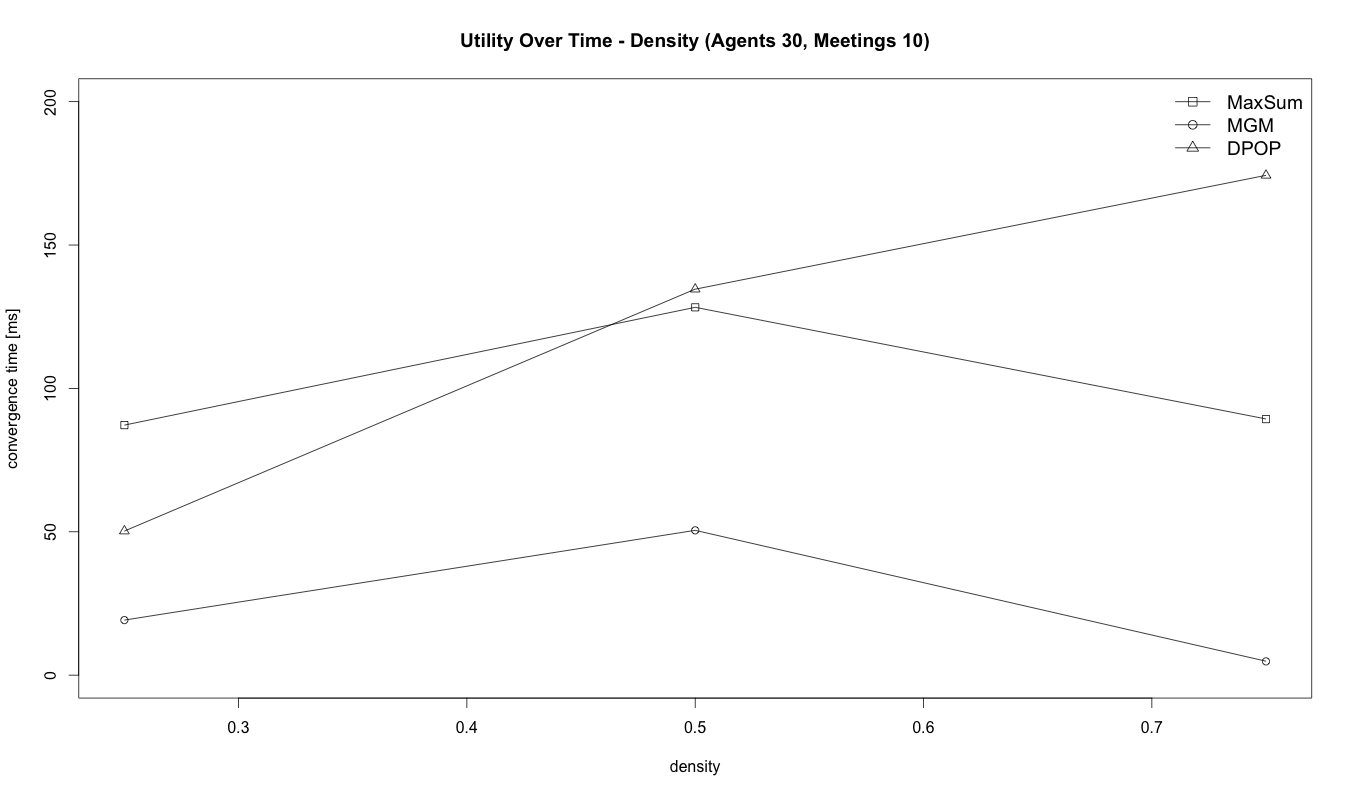
\includegraphics[width=330px]{graphics/experiments/static/st_18}
\caption{Utility over Time - Agents 30, Meetings 10}
\label{fig:st_18}
\end{figure}

% ----------------------------
A run with 10 Agents shows the expected effect of a problem density increase (Figure \ref{fig:st_17}). The benchmark with 30 agents again shows the case that MaxSum and MGM run comparably fast on 0.25 and 0.75, but have an increased convergence time on density value 0.5 (Figure \ref{fig:st_17}). DPOP does not scale the same way and increases significantly on density 0.75. This observation seems to be related to the local-iterative nature of MaxSum and MGM.
%-----------------------------


\section{Results II: Algorithms Performance in Dynamic Environments}

In this section, the benchmarks on dynamic abilities of the algorithms will be shown. Some parameters needed to be fixed during the benchmarks, as otherwise there would have been too many results to process. The test case has been 30 agents and 10 meetings.

\begin{figure}[H]
\centering
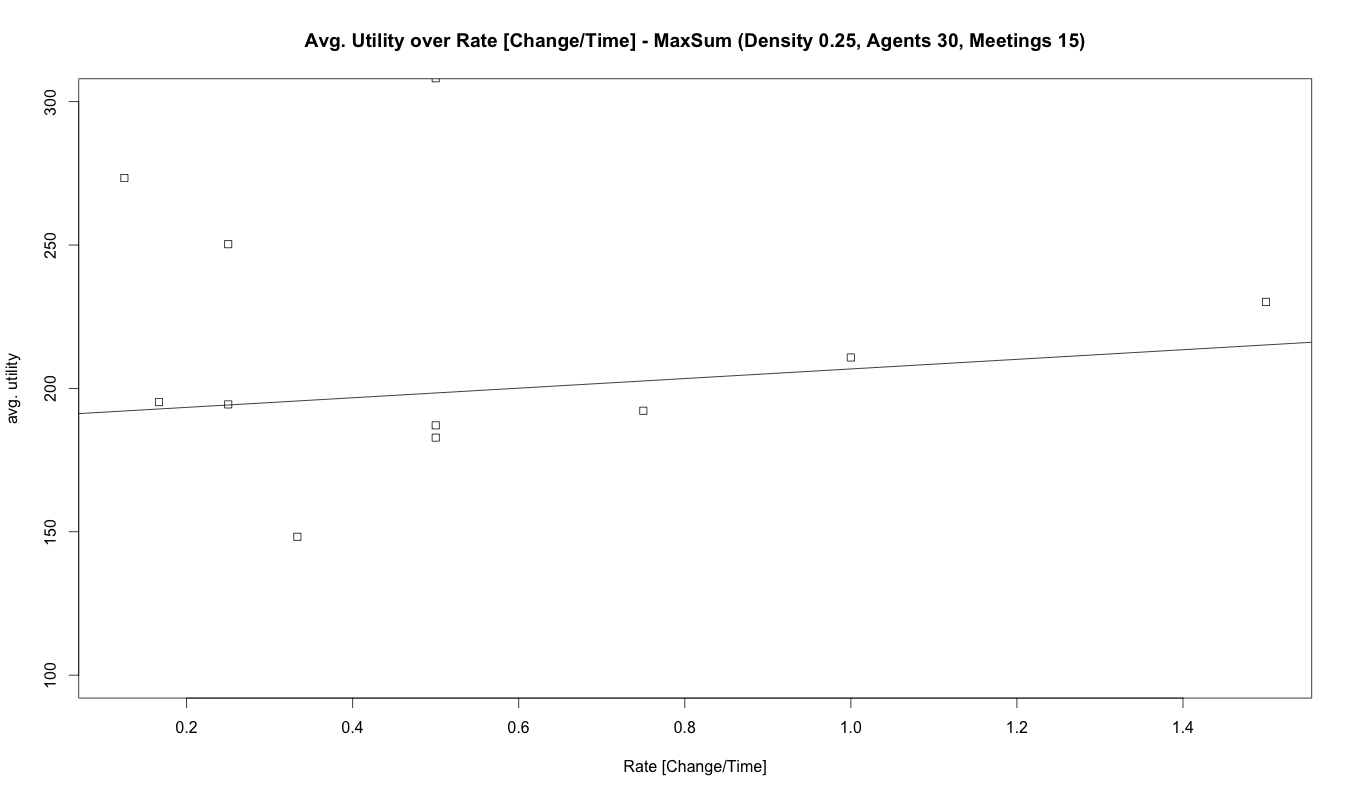
\includegraphics[width=330px]{graphics/experiments/dynamic/d_1.png}
\caption{Avg. Utility over Rate [Change/Time] - MaxSum}
\label{fig:d_1}
\end{figure}

One value for stability has been chosen to be change rate over average utility comparable to \cite{Maillera}. Instead of using the conflicts value, it was decided to use the utility value. The rate is defined as \(dP/dt\), whereas \(dP\) is the amount of change to constraints and \(dt\) is the difference in time. It was modelled to use different amounts of change. On can see in Figure \ref{fig:d_1} that the utility does increase over the 

EXTENSION HERE

\begin{figure}[H]
\centering
\begin{subfigure}{0.5\textwidth}
  \centering
  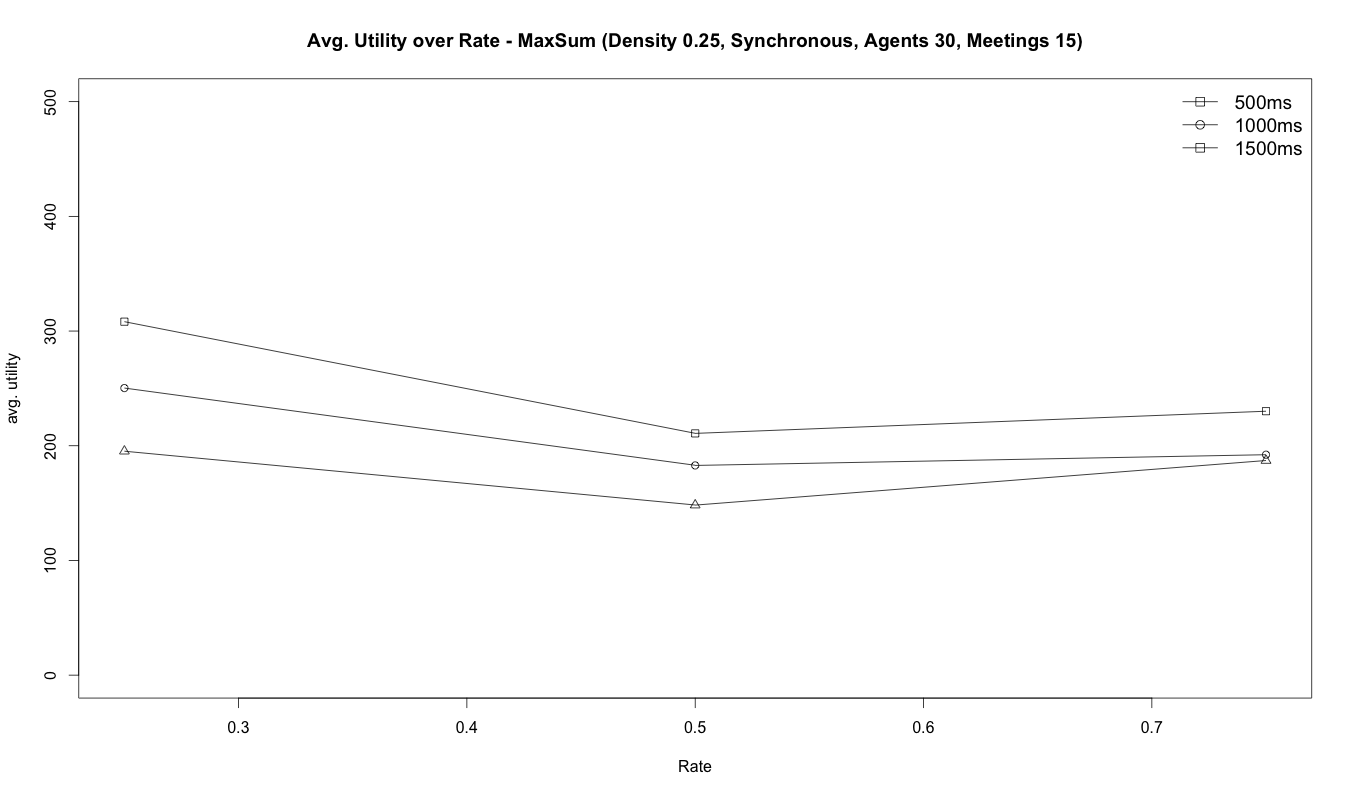
\includegraphics[width=1\linewidth]{graphics/experiments/dynamic/d_2.png}
  \caption{Avg. Utility over Rate - MaxSum - Synchronous}
  \label{fig:d_2}
\end{subfigure}%
\begin{subfigure}{0.5\textwidth}
  \centering
  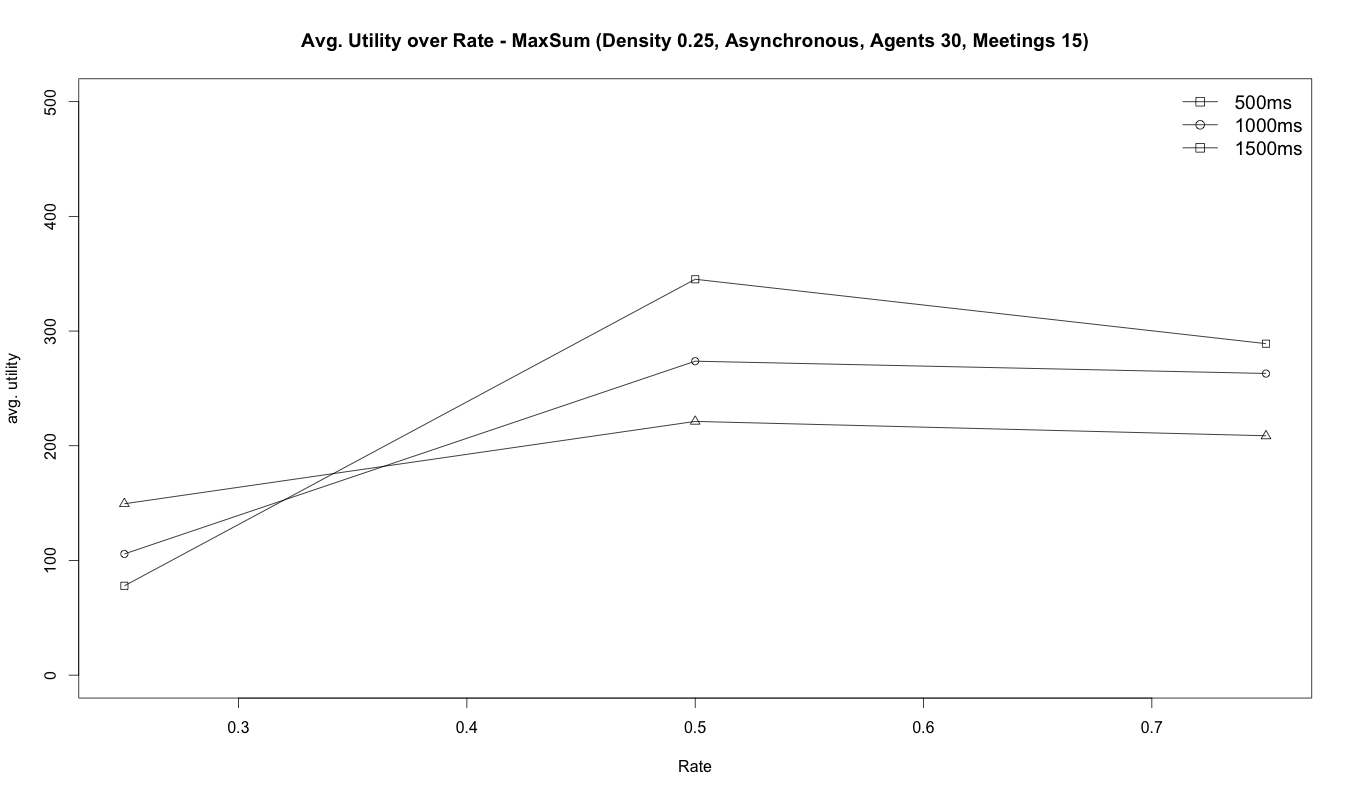
\includegraphics[width=1\linewidth]{graphics/experiments/dynamic/d_3.png}
  \caption{Avg. Utility over Rate - MaxSum - Asynchronous}
  \label{fig:d_3}
\end{subfigure}
\caption{Comparison of Avg. Utility over Rate - MaxSum - Asynchronous vs. Synchronous}
\label{fig:test}
\end{figure}

\begin{figure}[H]
\centering
\begin{subfigure}{0.5\textwidth}
  \centering
  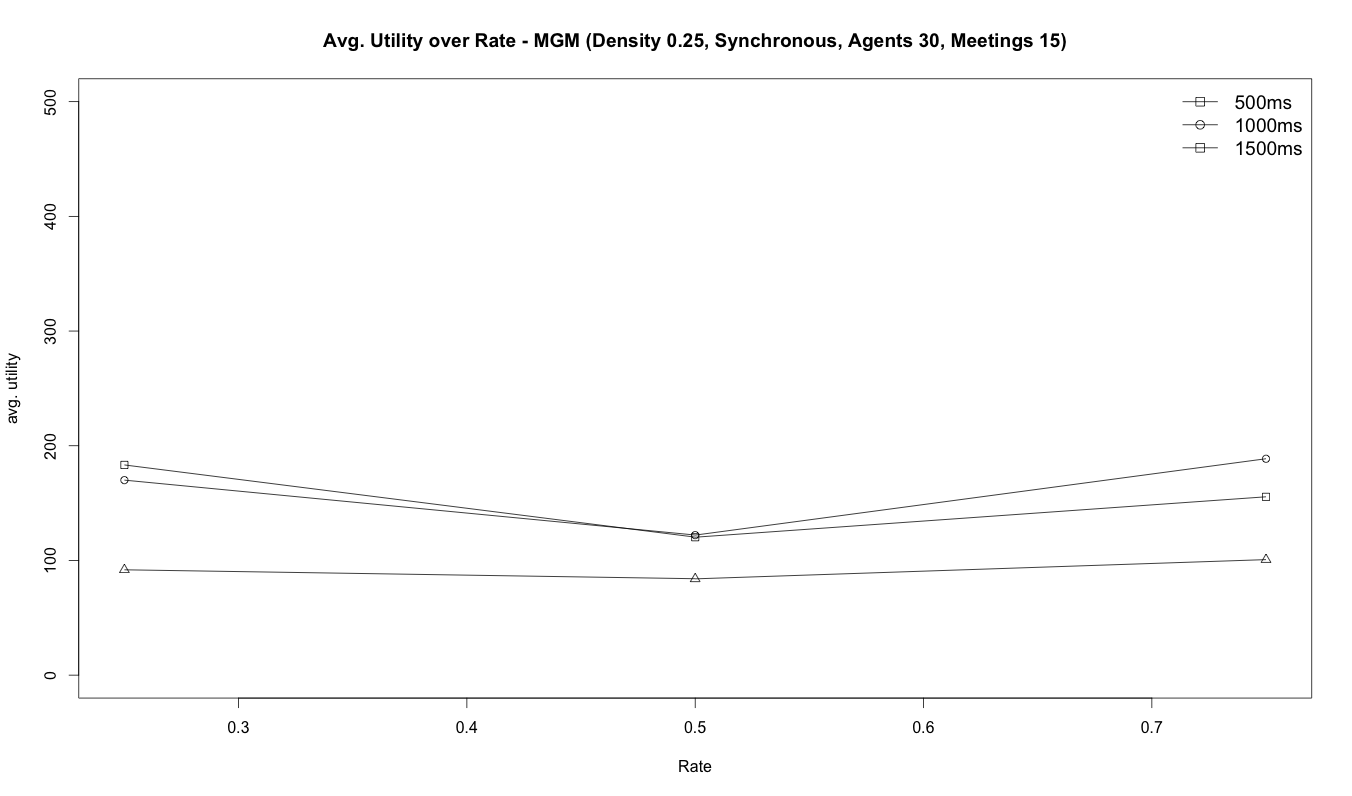
\includegraphics[width=1\linewidth]{graphics/experiments/dynamic/d_4.png}
  \caption{Avg. Utility over Rate - MGM - Synchronous}
  \label{fig:d_4}
\end{subfigure}%
\begin{subfigure}{0.5\textwidth}
  \centering
  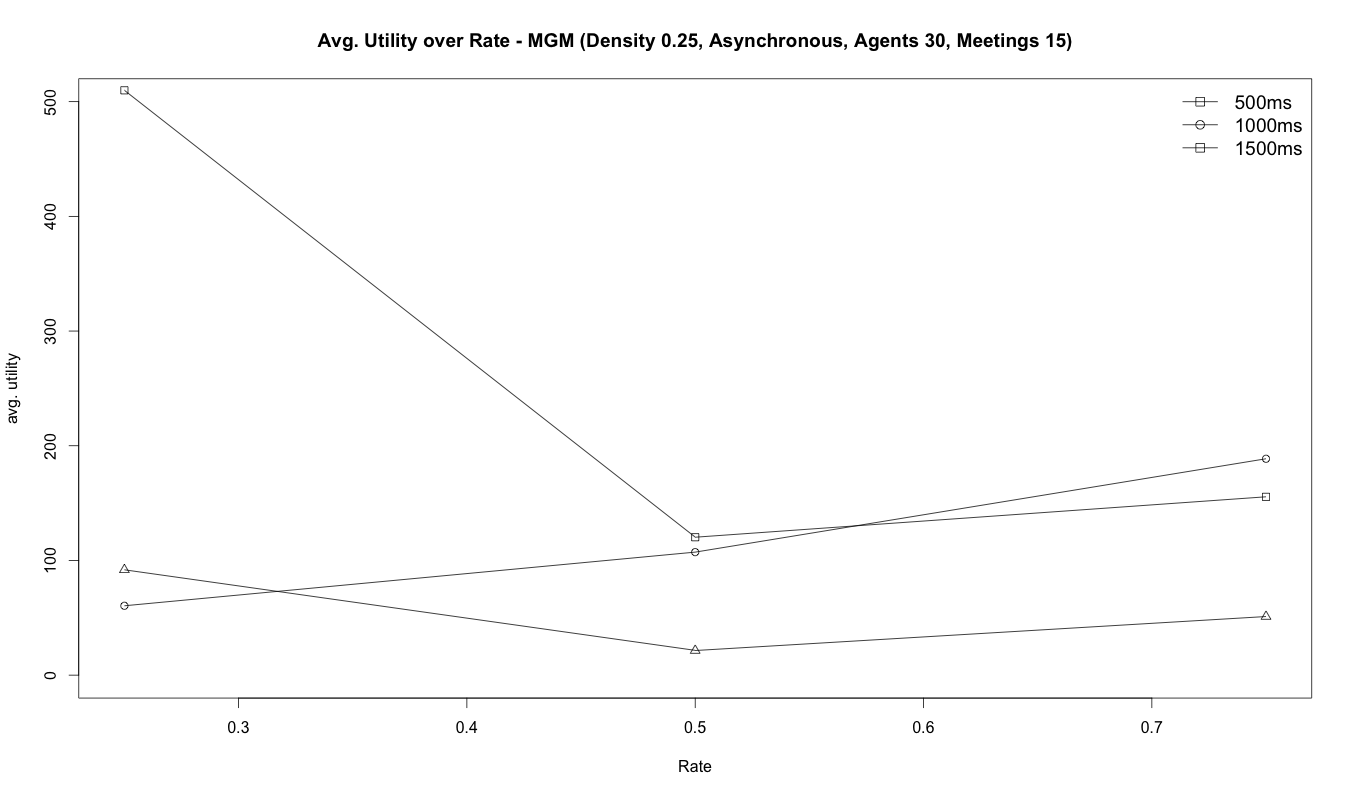
\includegraphics[width=1\linewidth]{graphics/experiments/dynamic/d_5.png}
  \caption{Avg. Utility over Rate - DPOP - Synchronous}
  \label{fig:d_5}
\end{subfigure}
\caption{Comparison of Avg. Utility over Rate - MGM - Synchronous vs. Asynchronous}
\label{fig:test}
\end{figure}

A further approach with Rate on the x-axis has been attempted, and it could be shown that MaxSum has the ability to handle various amounts of change well (Figures \ref{fig:d_2}, \ref{fig:d_3}. The synchronous mode does increase the performance significantly on change rate 0.5. MGM also does perform in a stable manner in the tested synchronous mode (Figure \ref{fig:d_4}). DPOP does not seem to be able to handle short intervals of change well as seen on value 500ms, but the algorithm shows stability on 1000ms and 1500ms change rates \ref{fig:d_5}.

TABLE HERE

DYNAMIC VARIABLES HERE





